\documentclass{ximera}
%%% You can put user macros here
%% However, you cannot make new environments

\listfiles

\graphicspath{{./}{firstExample/}{secondExample/}}

\usepackage{tikz}
\usepackage{tkz-euclide}
\usepackage{tikz-3dplot}
\usepackage{tikz-cd}
\usetikzlibrary{shapes.geometric}
\usetikzlibrary{arrows}
%\usetkzobj{all}
\pgfplotsset{compat=1.13} % prevents compile error.

%\renewcommand{\vec}[1]{\mathbf{#1}}
\renewcommand{\vec}{\mathbf}
\newcommand{\RR}{\mathbb{R}}
\newcommand{\dfn}{\textit}
\newcommand{\dotp}{\cdot}
\newcommand{\id}{\text{id}}
\newcommand\norm[1]{\left\lVert#1\right\rVert}
 
\newtheorem{general}{Generalization}
\newtheorem{initprob}{Exploration Problem}

\tikzstyle geometryDiagrams=[ultra thick,color=blue!50!black]

%\DefineVerbatimEnvironment{octave}{Verbatim}{numbers=left,frame=lines,label=Octave,labelposition=topline}



\usepackage{mathtools}


\author{Anna Davis} \title{MTH 140 Practice Problem} 

\begin{document}

\begin{abstract}

\end{abstract}
\maketitle
 \textit{You have 1 hour and 20 minutes to complete this test.  Each answer is worth 1 point.}
\begin{problem}\label{prob:test2prob1}
The diagram below shows two spinners.  (The arrow spins and points to one of three numbers.)  Two spinners are spun and the values are added together.  Let $X$ be the sum of the values.  

\begin{image}
   
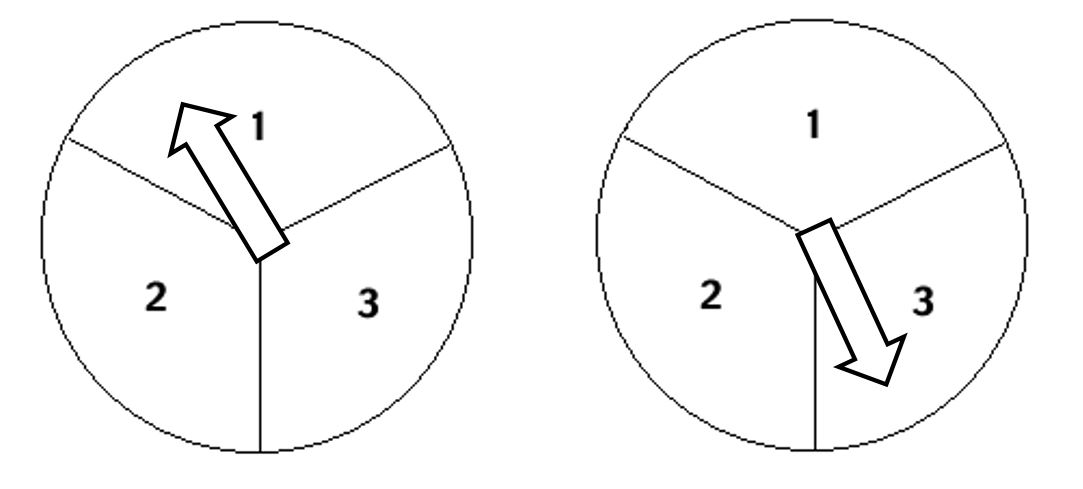
\includegraphics[height=1in]{test2pic1.jpg}~
 
\end{image}



\begin{enumerate}
    \item Fill out the following table to help you determine probabilities of obtaining various sums.
    
\begin{center}
\begin{tabular}{|c|c|c|c|}
 \hline
 && &   \\
 & $1$& $2$ &$3$ \\
 && &   \\
  \hline
  && & \\
 $1$&$\answer{2}$&$\answer{3}$&$\answer{4}$ \\
  &&& \\
 \hline
  &&& \\
 $2$&$\answer{3}$&$\answer{4}$ &$\answer{5}$ \\
  &&& \\
 \hline
  &&& \\
  $3$&$\answer{4}$&$\answer{5}$  &$\answer{6}$ \\
  &&& \\
 \hline
 \end{tabular}
\end{center}    
    
    
\item $$P(1)=\answer{0}$$ $$P(2)=\answer[tolerance=0.01]{\frac{1}{9}}$$ $$P(4)=\answer[tolerance=0.01]{\frac{1}{3}}$$ $$P(x<10)=\answer{1}$$ $$P(x\leq 4)=\answer[tolerance=0.01]{\frac{2}{3}}$$


\item Fill out the table provided below and find the expected value $(\mu)$ and the standard deviation $(\sigma)$.

\begin{center}
\begin{tabular}{|c|c|c|c|}
 \hline
 && &   \\
 Sum of Values ($x$) & $P(x)$& $xP(x)$ &$(x-\mu)^2P(x)$ \\
 && &   \\
  \hline
  && & \\
 \quad$2$\quad&$\answer[tolerance=0.01]{\frac{1}{9}}$&$\answer[tolerance=0.01]{\frac{2}{9}}$&$\answer[tolerance=0.01]{\frac{4}{9}}$ \\
  &&& \\
 \hline
  &&& \\
 \quad $3$&$\answer[tolerance=0.01]{\frac{2}{9}}$&$\answer[tolerance=0.01]{\frac{2}{3}}$ & $\answer[tolerance=0.01]{\frac{2}{9}}$ \\
  &&& \\
 \hline
  &&& \\
  \quad $4$&$\answer[tolerance=0.01]{\frac{1}{3}}$& $\answer[tolerance=0.01]{\frac{4}{3}}$ &$\answer[tolerance=0.01]{0}$ \\
  &&& \\
 \hline
  & &&\\
 \quad $5$& $\answer[tolerance=0.01]{\frac{2}{9}}$&$\answer[tolerance=0.01]{\frac{10}{9}}$  & $\answer[tolerance=0.01]{\frac{2}{9}}$\\
  &&&\\
 \hline
  & &&\\
 \quad $6$&$\answer[tolerance=0.01]{\frac{1}{9}}$ & $\answer[tolerance=0.01]{\frac{2}{3}}$ & $\answer[tolerance=0.01]{\frac{4}{9}}$\\
  &&&\\
 \hline
\end{tabular}
\end{center}
\vskip 0.5in
$$\mu=\answer{4};\quad \sigma =\answer[tolerance=0.01]{\frac{2}{\sqrt{3}}}$$
\end{enumerate}

\end{problem}



\end{document} 